%\section{Практична реалізація}
\section{ПРАКТИЧНА РЕАЛІЗАЦІЯ}

Даний розділ присвячується аналізу часового ряду тестувальної системи DOTS за допомогою мови програмування Python. 

Python $-$ це легка в освоєнні, потужна мова програмування. Він має ефективні структури даних високого рівня і простий, але ефективний підхід до об'єктно-орієнтованого програмування [7].

Python став загальноприйнятою мовою програмування для багатьох сфер застосування науки про дані. Дана мова програмування поєднує в собі міць мов програмування з простотою використання предметно орієнтованих скриптових мов типу MATLAB або R. 

В Python є бібліотеки для завантаження даних, візуалізації, статистичних обчислень, обробки природної мови, обробки зображень і багато чого іншого [8].

Також використовувався фреймфорк Anaconda. Це безкоштовний, включаючи комерційне використання, і готовий до використання в середовищі підприємства дистрибутив Python, який об'єднує всі ключові бібліотеки Python, необхідні для роботи в області науки про дані, математики та розробки, в одному зручному для користувача крос-платформенном дистрибутиві [9].

Для тренування нейронних мереж було обрано бібліотеку PyTorch. PyTorch - це бібліотека для програм Python, яка сприяє побудові проектів глибокого навчання [10].

Також використовувалась бібліотеки NumPy та matplotlib. NumPy є основним пакетом для наукових обчислень з Python [11]. Matplotlib $-$ це всебічна бібліотека для створення статичних, анімованих та інтерактивних візуалізацій у Python [12]. 

\subsection{Дані для аналізу}

Для демонстрації та аналізу роботи алгоритмів були використані дані з датасету CIFAR-10.

Набір даних CIFAR-10 складається з 60000 кольорових зображень розміром 32x32 у 10 класах, по 6000 зображень на клас. Існує 50000 навчальних зображень та 10000 тестових зображень [13].

Набір даних розділений на п’ять навчальних партій та одну тестову партію, кожна з 10000 зображень. Тестова партія містить рівно 1000 довільно обраних зображень з кожного класу. Навчальні партії містять решту зображень у довільному порядку, але деякі навчальні партії можуть містити більше зображень одного класу, ніж інші [13]. Навчальні партії містять рівно 5000 зображень від кожного класу.

Приклад зображень з датасету наведено у рис. \ref{fig:cifar10}.

\vspace{1em}

\begin{figure}[h]
  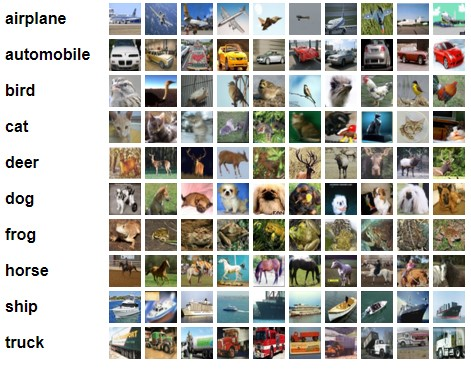
\includegraphics[width=\textwidth, height=3cm, natwidth=1227, natheight=187]{cifar10.jpg}
  \caption{Приклад зображень з датасету CIFAR-10}
  \label{fig:cifar10}
\end{figure}

\newpage

В базі даних є колонка $posted\_time$ $-$ це ціле число, яке відображає кількість мілісекунд від першого січня 1980 року. З циих чисел можна отримати дату відправлення до тестувальної системи. Після угрупування по датам отримуємо часовий ряд, наведений у рис. \ref{fig:TimeSeries}.


%Часовий ряд тестувальної системи DOTS має наступну структуру: в кожен день є певне ціле число відправлень, саме з цих чисел складається ряд. Часовий ряд наведено у рис. \ref{fig:TimeSeries}.

\vspace{1em}

\begin{figure}[h]
  \includegraphics[width=\textwidth, height=7cm, natwidth=854, natheight=476]{TimeSeries.jpg}
  \caption{Часовий ряд тестувальної системи DOTS}
  \label{fig:TimeSeries}
\end{figure}

Задля перевірки роботи алгоритму, часовий ряд було розділено на два ряди: тренувальний, та тестувальний. Будуть розглядати тренувальні ряди, які складають $90\%$ та $80\%$ від початкового, щоб побачити можливості алгоритмів для прогнозів разної тривалості.

\subsection{Аналіз та прогноз часового ряду за допомогою моделі ARIMA}
%\subsection{Аналіз та прогноз часового ряду з використанням моделі ARIMA}

У першому випадку, тренувальний ряд буде складати $90\%$ від початкового. У такому разі найбільш оптимальні параметри моделі ARIMA дорівнюють: $p = 6$, $d = 2$, $q = 4$. Результат прогнозування можна побачити на рис. \ref{fig:ARIMA90}.

\vspace{1em}

\begin{figure}[h]
  \includegraphics[width=\textwidth, height=7cm, natwidth=846, natheight=440]{ARIMA90.jpg}
  \caption{Порівняння оригінального та зпрогнозованого рядів}
  \label{fig:ARIMA90}
\end{figure}

%У табл. \ref{tab:ARIMA90} наведені параметри моделі та їхні до    вірчі інтервали.

Середня абсолютна процентна похибка (MAPE) дорівнює $17,84\%$, що є добрим прогнозом. У табл. \ref{tab:ARIMA90} наведені параметри моделі та їхні довірчі інтервали.

\begin{table}[h]
\caption{Довірні інтервали параметрів моделі}\label{tab:ARIMA90}
\begin{tabular}{|c|m{0.4\textwidth}|}
\hline
Параметр моделі & Довірчий інтервал \\
		\hlinewd{2pt}
$\alpha_{1} = -0,85$ & $-1,08 < -0,85 < -0,62$ \\
\hline
$\alpha_{2} = -0,93$ & $-1,13 < -0,93 < -0,72$ \\
\hline
$\alpha_{3} = -1,25$ & $-1,48 < -1,25 < -1,03$ \\
\hline
$\alpha_{4} = -0,94$ & $-1,14 < -0,94 < -0,75$ \\
\hline
$\alpha_{5} = -0,64$ & $-0,85 < -0,64 < -0,43$ \\
\hline
$\alpha_{6} = -0,45$ & $-0,62 < -0,45 < -0,28$ \\
\hline
$\theta_{1} = -0,98$ & $-1,12 < -0,98 < -0,84$ \\
\hline
$\theta_{2} = 0,34$ & $-0,04 < 0,34 < 0,65$ \\
\hline
$\theta_{3} = 0.45$ & $0.06 < 0.45 < 0.83$ \\
\hline
$\theta_{4} = -0,80$ & $-1,05 < -0,80 < -0,63$ \\
\hline
\end{tabular}
\end{table}

У випадку, коли тренувальний ряд дорівнює $80\%$ від початкового, то можемо бачити результати на рис. \ref{fig:ARIMA80}.

\newpage

\vspace{1em}

\begin{figure}[h]
  \includegraphics[width=\textwidth, height=7cm, natwidth=843, natheight=448]{ARIMA80.jpg}
  \caption{Порівняння оригінального та зпрогнозованого рядів}
  \label{fig:ARIMA80}
\end{figure}

Середня абсолютна процентна похибка (MAPE) дорівнює $45,94\%$, що є добрим прогнозом. У табл. \ref{tab:ARIMA80} наведені параметри моделі та їхні довірчі інтервали.

\begin{table}[h]
\caption{Довірні інтервали параметрів моделі}\label{tab:ARIMA80}
\begin{tabular}{|c|m{0.4\textwidth}|}
\hline
Параметр моделі & Довірчий інтервал \\
		\hlinewd{2pt}
$\alpha_{1} = -0,99$ & $-1,22 < -0,99 < -0,75$ \\
\hline
$\alpha_{2} = -1,08$ & $-1,31 < -1,08 < -0,85$ \\
\hline
$\alpha_{3} = -1,39$ & $-1,63 < -1,39 < -1,14$ \\
\hline
$\alpha_{4} = -1,08$ & $-1,30 < -1,08 < -0,85$ \\
\hline
$\alpha_{5} = -0,75$ & $-0,97 < -0,75 < -0,52$ \\
\hline
$\alpha_{6} = -0,52$ & $-0,69 < -0,52 < -0,34$ \\
\hline
$\theta_{1} = -0,88$ & $-1,11 < -0,88 < -0,64$ \\
\hline
$\theta_{2} = 0,28$ & $-0,08 < 0,28 < 0,64$ \\
\hline
$\theta_{3} = 0,43$ & $0.04 < 0.43 < 0.82$ \\
\hline
$\theta_{4} = -0,83$ & $-1,04 < -0,83 < -0,62$ \\
\hline
\end{tabular}
\end{table}

\subsection{Аналіз та прогноз часового ряду за допомогою алгоритму SSA}

У випадку алгоритму SSA будемо тестувати різні довжини вікон.

Якщо довжина вікна дорівнює $10$, та тренувальний ряд складає $90\%$ оригінального, то отримуємо результати приведені у рис. \ref{fig:SSA9010}.

\vspace{1em}

\begin{figure}[h]
  \includegraphics[width=\textwidth, height=6cm, natwidth=872, natheight=447]{SSA9010.jpg}
  \caption{Порівняння оригінального та зпрогнозованого рядів}
  \label{fig:SSA9010}
\end{figure}

В такому випадку $\text{MAPE} = 37,04\%$.

Якщо довжина вікна дорівнює $17$, та тренувальний ряд складає $90\%$ оригінального, то отримуємо результати приведені у рис. \ref{fig:SSA9016}.

\vspace{1em}

\begin{figure}[h]
  \includegraphics[width=\textwidth, height=7cm, natwidth=880, natheight=447]{SSA9016.jpg}
  \caption{Порівняння оригінального та зпрогнозованого рядів}
  \label{fig:SSA9016}
\end{figure}

1-а власна трійка приведена на рис. \ref{fig:Trend90} відповідає тренду:

\newpage

\vspace{1em}

\begin{figure}[h]
  \includegraphics[width=\textwidth, height=7cm, natwidth=822, natheight=408]{Trend90.jpg}
  \caption{Трендова складова}
  \label{fig:Trend90}
\end{figure}

2-а власна трійка є сезонною складовою. Її приведено на рис. \ref{fig:Cyclic190}.

\vspace{1em}

\begin{figure}[h]
  \includegraphics[width=\textwidth, height=7cm, natwidth=817, natheight=410]{Cyclic190.jpg}
  \caption{Перша сезонна складова}
  \label{fig:Cyclic190}
\end{figure}

Як можна побачити з графіку, 3-я власна трійка є також сезонною складовою. Її приведено на рис. \ref{fig:Cyclic290}.

\newpage

\vspace{1em}

\begin{figure}[h]
  \includegraphics[width=\textwidth, height=7cm, natwidth=820, natheight=411]{Cyclic290.jpg}
  \caption{Друга сезонна складова}
  \label{fig:Cyclic290}
\end{figure}


Якщо подивитися на двовимірну діаграму між 14 та 15 власними трійками, приведену на рис. \ref{fig:Diag90}, можна зробити висновок, що всі власні трійки після 14 відповідають за шумові процеси і їх можна не розглядати.


\vspace{1em}

\begin{figure}[h]
  \includegraphics[width=\textwidth, height=7cm, natwidth=837, natheight=422]{Diag90.jpg}
  \caption{Двовимірна діаграма 14 і 15 власних трійок}
  \label{fig:Diag90}
\end{figure}

В такому випадку $\text{MAPE} = 29,68\%$. Експерементальним шляхом було визначено, що дане значення є оптимальним.

Якщо довжина вікна дорівнює $10$, та тренувальний ряд складає $80\%$ оригінального, то отримуємо результати приведені у рис. \ref{fig:SSA8010}.

\newpage

\vspace{1em}

\begin{figure}[h]
  \includegraphics[width=\textwidth, height=7cm, natwidth=876, natheight=436]{SSA8010.jpg}
  \caption{Порівняння оригінального та зпрогнозованого рядів}
  \label{fig:SSA8010}
\end{figure}

В такому випадку $\text{MAPE} = 47.59\%$.

Якщо довжина вікна дорівнює $11$, та тренувальний ряд складає $80\%$ оригінального, то отримуємо результати приведені у рис. \ref{fig:SSA8011}.

\begin{figure}[h]
  \includegraphics[width=\textwidth, height=7cm, natwidth=868, natheight=435]{SSA8011.jpg}
  \caption{Порівняння оригінального та зпрогнозованого рядів}
  \label{fig:SSA8011}
\end{figure}

В такому випадку $\text{MAPE} = 40.22\%$. Експерементальним шляхом було визначено, що дане значення є оптимальним.

\subsection{Висновки за розділом}

В даному розділі була продемонстрована робота алгоритмів Deep InfoMax та Momentum Contrast. БУли реалізовані програми мовою програмування Python за допомогою спеціальних бібліотек для аналізу даних та програмного фреймворку Anaconda. 

Як видно з результатів, модель Deep InfoMax дає якісніший прогноз, в той час як алгоритм Momentum Contrast потребує менше часових та обчислювальних ресурсів.
